
It is quite common that at some point one must answer the question:
"Given a mesh and its connectivity on the one hand, and the coordinates of a 
point on the other, how do I accurately and quickly determine in which element 
the point resides?"

One typical occurence of such a problem is linked to the use of the Particle-In-Cell 
technique: particles are advected and move through the mesh, and need to be localised 
at every time step. This question could arise in the context of a benchmark where 
certain quantities need to be measured at specific locations inside the domain. 

%-------------------------------------------
%-------------------------------------------
\subsubsection{Two-dimensional space}

We shall first focus on quadrilaterals. There are many kinds of quadrilaterals as shown 
hereunder: 

\begin{center}
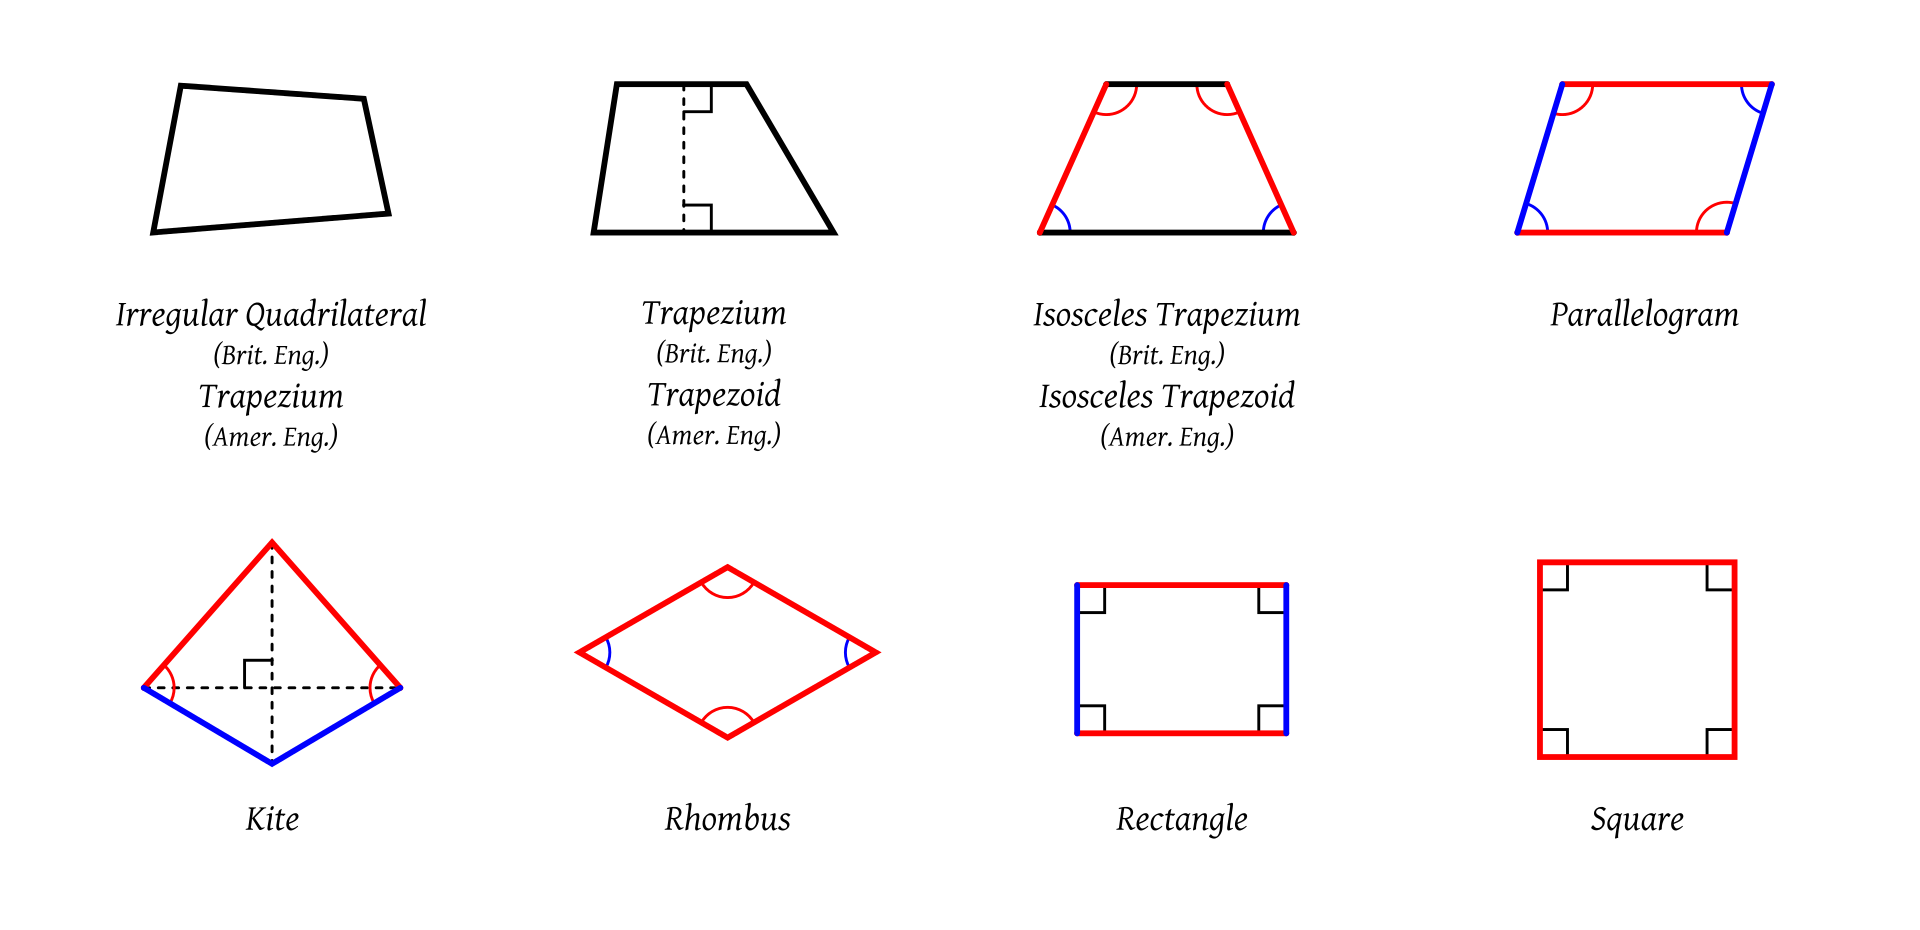
\includegraphics[width=12cm]{images/quadrilaterals} \\
{\captionfont from Wikipedia \url{https://en.wikipedia.org/wiki/Quadrilateral#/media/File:Quadrilaterals.svg}}
\end{center}



%..................................................
\paragraph{The trivial case of rectangular elements} 

Testing whether the point $M$ is inside the element is trivial. Its reduced coordinates
are given by
\begin{eqnarray}
r_M &=& \frac{2}{x_2-x_0}(x_M-x_0) -1 = \frac{2}{h_x}(x_M-x_0)-1  \\
s_M &=& \frac{2}{y_2-y_0}(y_M-y_0) -1 = \frac{2}{h_y}(y_M-y_0)-1  
\end{eqnarray}

\begin{center}
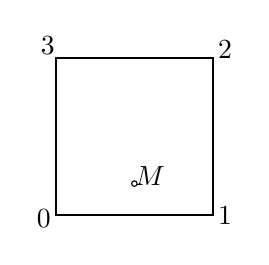
\begin{tikzpicture}
%\draw[step=0.5cm,gray,very thin] (0,0) grid (4,4); %background grid
\draw[thick] (1,1) -- (3,1) -- (3,3) -- (1,3) -- cycle;  
\node[] at (0.85,0.95) {0};
\node[] at (3.15,1) {1};
\node[] at (3.15,3.1) {2};
\node[] at (0.9,3.15) {3};
\node[] at (2.2,1.5) {$M$};
\draw (2.,1.4) circle (1pt);
\end{tikzpicture}\\
\end{center}


%..................................................
\paragraph{An intermediate case} We make the following assumption that the lateral sides of the  
element are vertical while the bottom and top are not necessarily horizontal:

\begin{center}
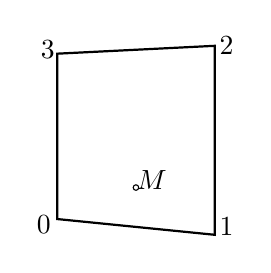
\begin{tikzpicture}
%\draw[step=0.5cm,gray,very thin] (0,0) grid (4,4); %background grid
\draw[thick] (1,1) -- (3,0.8) -- (3,3.2) -- (1,3.1) -- cycle;  
\node[] at (0.83,0.93) {0};
\node[] at (3.15,0.9) {1};
\node[] at (3.15,3.2) {2};
\node[] at (0.88,3.15) {3};
\node[] at (2.2,1.5) {$M$};
\draw (2.,1.4) circle (1pt);
\end{tikzpicture}\\
\end{center}

Because the sides are verical then if $x_0 \leq x_M \leq x_2$ then 
\[
r_M = \frac{2}{x_2-x_0}(x_M-x_0) -1 
\]
Then, if $M$ is inside the element then its $y$ coordinate is given by
\[
y_M = \sum_i N_i(r_M,s_M) y_i
\]
where $N_i$ are the four $Q_1$ shape functions associated to the vertices.
Assuming we know $r_M$ then we can solve for $s_M$:
\begin{eqnarray}
y_M &=&  
\frac{1}{4}(1-r_M)(1-s_M) y_0+
\frac{1}{4}(1+r_M)(1-s_M) y_1+
\frac{1}{4}(1+r_M)(1+s_M) y_2+
\frac{1}{4}(1-r_M)(1+s_M) y_3 \nn\\
&=& 
\frac{1}{4} \left[
(1-r)y_0+(1+r)y_1+(1+r)y_2+(1-r)y_3 +s_M [ -(1-r)y_0 - (1+r)y_1+(1+r)y_2+(1-r)y_3  ] 
\right] \nn 
\end{eqnarray}
or, 
\[
s_M = \frac{ 4y_M - [(1-r_M)y_0+(1+r_M)y_1+(1+r_M)y_2+(1-r_M)y_3]  }{ -(1-r_M)y_0 -(1+r_M)y_1+(1+r_M)y_2+(1-r_M)y_3 } 
\]
If the obtained value is in $[-1,1]$ then the point $M$ is in the element.
Verification: when $y_1=y_0$ and $y_2=y_3$ then 
\begin{eqnarray}
s_M 
&=& \frac{4 y_M - [(1-r_M)y_0+(1+r_M)y_0+(1+r_M)y_3+(1-r_M)y_3]  }{ -(1-r_M)y_0 - (1+r_M)y_0+(1+r_M)y_3+(1-r_M)y_3 } \nn\\
&=& \frac{4 y_M - [ 2 y_0 + 2 y_3]  }{ -2 y_0 + 2 y_3    }  \nn\\
&=& \frac{1}{y_3-y_0} [2 y_M - (  y_0 +  y_3) ] \nn\\ 
&=& \frac{1}{y_3-y_0} [2 y_M -  2 y_0 +y_0 -  y_3)  ] \nn\\ 
&=& \frac{2}{y_3-y_0} (y_M - y_0) - 1 
\end{eqnarray}
which is the expression that corresponds to a rectangular element as seen previously.

%..................................................
\paragraph{A generic quadrilateral}

We wish to arrive at a single algorithm which is applicable to all quadrilaterals and we now focus  
on an irregular quadrilateral (no face is parallel to the axis of the coordinate system). 

\begin{center}
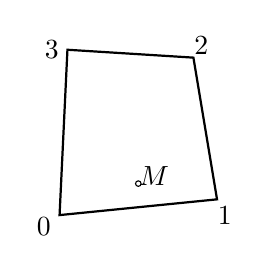
\begin{tikzpicture}
%\draw[step=0.5cm,gray,very thin] (0,0) grid (4,4); %background grid
\draw[thick] (1,1) -- (3,1.2) -- (2.7,3) -- (1.1,3.1) -- cycle;  
\node[] at (0.8,0.85) {0};
\node[] at (3.1,1) {1};
\node[] at (2.8,3.15) {2};
\node[] at (0.9,3.1) {3};
\node[] at (2.2,1.5) {$M$};
\draw (2.,1.4) circle (1pt);
\end{tikzpicture}\\
\end{center}

Several rather simple options exist:
\begin{itemize}
\item we could subdivide the quadrilateral into two triangles and check whether point $M$ is inside any of them (as it turns out, 
this problem is rather straightforward for triangles. Simply google it.)
\item We could check that point $M$ is always on the left side of segments $0\rightarrow 1$, $1\rightarrow 2$, $2\rightarrow 3$, $3\rightarrow 0$.
\item ...  
\end{itemize}

Any of these approaches will work although some might be faster than others. In three-dimensions all will however become 
cumbersome to implement and might not even work at all. Fortunately, there is an elegant way to answer the question, as 
detailed in the following subsection, which works both in 2D and 3D.

%-------------------------------------------
\subsubsection{Three-dimensional space}

If point $M$ is inside the quadrilateral, there exist a set of reduced coordinates $r,s,t\in[-1:1]^3$ such that 

\[
\sum_{i=1}^4 N_i(r_M,s_M,t_M) x_i = x_M
\quad\quad\quad
\sum_{i=1}^4 N_i(r_M,s_M,t_M) y_i = y_M
\quad\quad\quad
\sum_{i=1}^4 N_i(r_M,s_M,t_M) z_i = z_M
\]
This can be cast as a system of three equations and three unknowns. Unfortunately, each shape function $N_i$ 
contains a term $rst$ (as well as $rs$, $rt$, and $st$) so that it is not a linear system and standard techniques
are not applicable. 
We must then use an iterative technique: the algorithm starts with a guess for values $r_M,s_M,t_M$ and 
improves on their value iteration after iteration. In what follows the subscript $M$ is dropped from $r,s,t$.

The classical way of solving nonlinear systems of equations is Newton's method. 
\index{general}{Newton's method}
We can rewrite the equations above as ${\bm F}(r,s,t)=0$:
\begin{eqnarray}
\sum_{i=1}^8 N_i(r,s,t) x_i - x_M&=&0 \nonumber\\
\sum_{i=1}^8 N_i(r,s,t) y_i - y_M&=&0 \nonumber\\
\sum_{i=1}^8 N_i(r,s,t) z_i - z_M&=&0
\end{eqnarray}
or,
\begin{eqnarray}
F_r(r,s,t)&=&0 \nonumber\\
F_s(r,s,t)&=&0 \nonumber\\
F_t(r,s,t)&=&0 \nonumber
\end{eqnarray}

so that we now have to find the zeroes of continuously differentiable functions ${\bm F}:\mathbb{R} \rightarrow \mathbb{R}$.
The recursion is simply:
\[
\left(
\begin{array}{c}
r_{k+1} \\s_{k+1} \\ t_{k+1}
\end{array}
\right)
=
\left(
\begin{array}{c}
r_{k} \\s_{k} \\ t_{k}
\end{array}
\right)
- J_F(r_k,s_k,t_k) ^{-1} 
\left(
\begin{array}{c}
F_r(r_k,s_k,t_k) \\
F_s(r_k,s_k,t_k)\\
F_t(r_k,s_k,t_k)
\end{array}
\right)
\]
where $J$ the Jacobian matrix:
\begin{eqnarray}
J_F(r_k,s_k,t_k)
&=&
\left(
\begin{array}{ccc}
\frac{\partial F_r}{\partial r}(r_k,s_k,t_k) & \frac{\partial F_r}{\partial s}(r_k,s_k,t_k) & \frac{\partial F_r}{\partial t}(r_k,s_k,t_k) \\\\
\frac{\partial F_s}{\partial r}(r_k,s_k,t_k) & \frac{\partial F_s}{\partial s}(r_k,s_k,t_k) & \frac{\partial F_s}{\partial t}(r_k,s_k,t_k) \\\\
\frac{\partial F_t}{\partial r}(r_k,s_k,t_k) & \frac{\partial F_t}{\partial s}(r_k,s_k,t_k) & \frac{\partial F_t}{\partial t}(r_k,s_k,t_k) 
\end{array}
\right) \nonumber\\
&=&
\left(
\begin{array}{ccc}
\sum\limits_{i=1}^8 \frac{\partial N_i}{\partial r}(r_k,s_k,t_k) x_i &
\sum\limits_{i=1}^8 \frac{\partial N_i}{\partial s}(r_k,s_k,t_k) x_i &
\sum\limits_{i=1}^8 \frac{\partial N_i}{\partial t}(r_k,s_k,t_k) x_i \\
\sum\limits_{i=1}^8 \frac{\partial N_i}{\partial r}(r_k,s_k,t_k) y_i &
\sum\limits_{i=1}^8 \frac{\partial N_i}{\partial s}(r_k,s_k,t_k) y_i &
\sum\limits_{i=1}^8 \frac{\partial N_i}{\partial t}(r_k,s_k,t_k) y_i \\
\sum\limits_{i=1}^8 \frac{\partial N_i}{\partial r}(r_k,s_k,t_k) z_i &
\sum\limits_{i=1}^8 \frac{\partial N_i}{\partial s}(r_k,s_k,t_k) z_i &
\sum\limits_{i=1}^8 \frac{\partial N_i}{\partial t}(r_k,s_k,t_k) z_i 
\end{array}
\right) \nonumber 
\end{eqnarray}
In practice, we solve the following system:
\[
J_F(r_k,s_k,t_k) 
\left[  
\left(
\begin{array}{c}
r_{k+1} \\s_{k+1} \\ t_{k+1}
\end{array}
\right)
-
\left(
\begin{array}{c}
r_{k} \\s_{k} \\ t_{k}
\end{array}
\right)
\right]=-
\left(
\begin{array}{c}
F_r(r_k,s_k,t_k) \\
F_s(r_k,s_k,t_k)\\
F_t(r_k,s_k,t_k)
\end{array}
\right)
\]
Finally, the algorithm goes as follows:
\begin{itemize}
\item set guess values for $r,s,t$ (typically 0)
\item loop over k=0,...
\item Compute rhs= $-{\bm F}(r_k,s_k,t_k)$ 
\item Compute matrix $J_F(r_k,s_k,t_k)$
\item solve system for $(dr_k,ds_k,dt_k)$
\item update $r_{k+1}=r_k+dr_k$, $s_{k+1}=s_k+ds_k$, $t_{k+1}=t_k+dt_k$ 
\item stop iterations when $(dr_k,ds_k,dt_k)$ is small
\item if $r_k,s_k,t_k\in[-1,1]^3$ then $M$ is inside.
\end{itemize}
This method converges quickly but involves iterations, and multiple solves of $3\times 3$ systems which, 
when carried out for each marker and at each time step can prove to be expensive. 
A simple modification can be added to the above algorithm: iterations should be carried out {\it only}
when the point $M$ is inside of a cuboid of size $[\min\limits_i{x_i}:\max\limits_i{x_i}]\times[\min\limits_i{y_i}:\max\limits_i{y_i} ]
\times[\min\limits_i{z_i}:\max\limits_i{z_i}]$ where the sums run over the vertices of the element. 
In 2D this translates as follows: only carry out Newton iterations when $M$ is inside the red rectangle!
\begin{center}
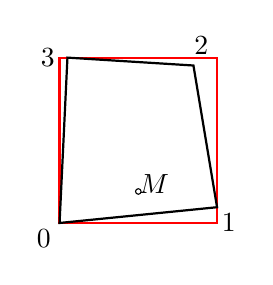
\begin{tikzpicture}
%\draw[step=0.5cm,gray,very thin] (0,0) grid (4,4); %background grid
\draw[thick,red] (1,1) -- (3,1) -- (3,3.1) -- (1,3.1) -- cycle;  
\draw[thick] (1,1) -- (3,1.2) -- (2.7,3) -- (1.1,3.1) -- cycle;  
\node[] at (0.8,0.8) {0};
\node[] at (3.15,1) {1};
\node[] at (2.8,3.25) {2};
\node[] at (0.85,3.1) {3};
\node[] at (2.2,1.5) {$M$};
\draw (2.,1.4) circle (1pt);
\end{tikzpicture}\\
\end{center}

Note that the algorithm above extends to high degree elements such as $Q_2$ and higher, even with curved sides.
As shown in the 2D case if the element is a cuboid or if all its lateral faces are vertical then one can 
compute the reduced coordinates without using an iterative method.



